\subsection{Origin of the Degeneracy}\label{sec:origin-of-degeneracy}
The fact that the spin representation $\mathcal{S}$ and the Majorana representation $\mathcal{M}$ are identical implies that the reduced density matrix might have a block-diagonal structure, in which the blocks are all identical. However, this is only a hypothesis instead of a direct and rigorous proof of the existence of such a structure. To see that the density matrix indeed has such a block-diagonal structure, we have to find the operator corresponding to each block that commutes with the density matrix. In addition, to make every block identical, there must be operators that provide equivalence relations among blocks.

In light of the physical pictures given by \cite{Yao-Qi} and \cite{PRX-ent-high}, it turns out that the operators are defined at the boundary of the subregion because the block-diagonal structure of the reduced density matrix is due to the Gauss law of the gauge field~\cite{PRX-ent-high}. Suppose the Gauss law in a gauge theory defined on a lattice is $\sum_{j\in N_i}E_{ij} = \rho_i$, where $\rho_i$ is the matter field on the lattice site $i$, $E_{ij}$ is the electric field residing on the edge $\anglelr{ij}$, and $N_i$ is the set of nearest neighbors of the site $i$. Because the boundary of the chosen subregion \textit{splits} the Gauss law of some neighborhoods $N_i$ that cross the boundary, making some edges in the environment and others in the subregion, it causes entanglement between the subregion and the environment. More precisely, the gauge-field operators in the chosen region and are separated from gauge-field operators and the corresponding matter fields in the environment by the boundary, which afterward act as symmetry operators that block-diagonalize the reduced density matrix. 

In the Kitaev model, the gauge theory is emergent due to the Majorana representation of the spin operators. Thus, the Gauss law of the gauge theory in the Kitaev model, which reads $b^x_ib^y_ib^z_ic_i = \mathds{1}$, only exists in the Majorana representation. Another issue is that the fundamental degrees of freedom of the Kitaev model reside on the lattice sites of the lattice, but the electric field operators $E_{ij}$ of the gauge theory, defined by $\mrm{e}^{i E_{ij}} = b^{\alpha_{ij}}_i$, live on edges, and which are not well-defined in the original setting of the model. For these reasons, we cannot directly apply the method proposed from~\cite{PRX-ent-high}. Some modifications are necessary.

Our solution to this issue is to transform a Majorana fermion theory coupled to a gauge field back to the physical spin representation by \textit{gluing} pairs of fermions using string operators. As we have noted earlier, the residual electric field inside the subregion after tracing out the environment is proportional to the exponent of $b$-Majorana fermions at the boundary, with the direction pointing outward. For simplicity, say, there are an even number $\abs{\de A} = 2L$ of edges crossing the boundary of the simply-connected region $A$, then the set of $b$-Majorana fermions encoding the residual electric field is $\lrg{b^{\mu_1}_{i_1}, b^{\mu_2}_{i_2}, b^{\mu_3}_{i_3},\cdots,b^{\mu_{2L}}_{i_{2L}}}$, in which $\mu_k$ stands for the direction of the $k$-th edge, which is connected to site $i_k$, that crosses the boundary. Notice that the necessary and sufficient condition to have $\abs{\de A}$ an even number is that the number of lattice sites $N^A$ in $A$ is also an even number. This fact can be seen directly from equation \eqref{equ.Pick_sim-con} relating $N^A$, $N^A_p$, and $\abs{\de A}$, in which the term $2N^A_p$ is always an even number, hence 
\begin{equation}\label{equ.bulk-boundary-parity}
    N^A=\abs{\de A}\mod{2}.
\end{equation}
To transform these $b$-Majorana fermions to a physical representation, we insert gauge-field operators along strings $\mathcal{C}_1, \mathcal{C}_2, \mathcal{C}_3,\cdots, \mathcal{C}_{L}$ that link pairs of Majorana fermions $(b^{\mu_1}_{i_1},b^{\mu_2}_{i_2}), (b^{\mu_3}_{i_3},b^{\mu_4}_{i_4}),\cdots,(b^{\mu_{2L-1}}_{i_{2L-1}},b^{\mu_{2L}}_{i_{2L}})$, respectively, to create a series of physical operators of the form
\begin{equation}\label{equ.b-link}
    b^{\mu_{2n-1}}_{i_{2n-1}} \lr{\prod_{\anglelr{ij}\in\mathcal{C}_{n}} \hat{u}_{ij}}b^{\mu_{2n}}_{i_{2n}} \quad ; \quad n=1,2,3,\cdots, L
\end{equation}
in which the two $b$-Majorana fermions $b^{\mu_{2n-1}}_{i_{2n-1}}$ and $b^{\mu_{2n}}_{i_{2n}}$ are at the endpoints of the string $\mathcal{C}_n$, and the product of gauge-field operators in between is the string that links the two endpoints together. 
\begin{figure}
    \centering
    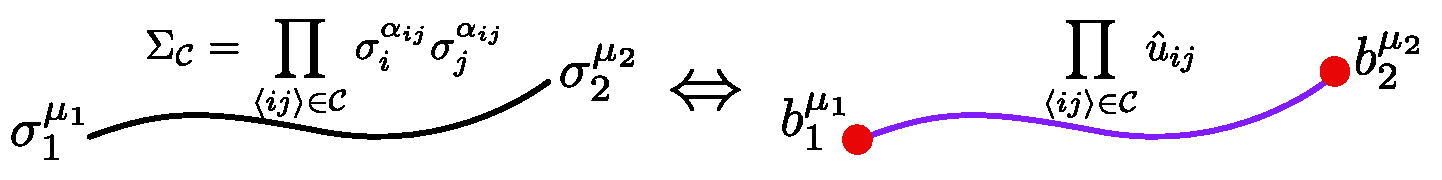
\includegraphics[width=\linewidth]{figures/linking-string-electric-field.pdf}
    \caption{Two $b$-Majorana fermions can also be linked by a series of gauge-field operators, $\prod_{\anglelr{ij}\in\mathcal{C}} \hat{u}_{ij}$. In that way, a physical operator $\xi$ is constructed.}
    \label{fig.linking-strings-electric-field}
\end{figure}
However, the expression \eqref{equ.b-link} only contains $b$-Majorana fermions and cannot be transformed directly to the spin representation. To obtain physical strings containing purely spin operators, we can further insert $c$-Majorana fermions into expression \eqref{equ.b-link}, then we obtain the following result   
\begin{equation}\label{equ.c-b-link}
    b^{\mu_{2n-1}}_{i_{2n-1}}c_{i_{2n-1}} \lr{\prod_{\anglelr{ij}\in\mathcal{C}_{n}} c_i\hat{u}_{ij}c_j}c_{i_{2n}}b^{\mu_{2n}}_{i_{2n}}
\end{equation}
in which those inserted $c$-Majorana fermions are identities $cc=\mathds{1}$, thus everything remains the same. After considering the transformation $\sigma^\mu_i\to ib^\mu_ic_i$, the operator \eqref{equ.c-b-link} is equal to the operators $\xi_n$ defined in the following way
\begin{equation}\label{equ.spin-string-linking-gauge}
    \xi_n \equiv \sigma^{\mu_{2n-1}}_{i_{2n-1}}\Sigma_{\mathcal{C}_n}\sigma^{\mu_{2n}}_{i_{2n}} \quad ; \quad n=1,2,3,\cdots ,L
\end{equation}
up to a phase that depends on the lengths of the strings $\abs{\mathcal{C}_n}$. The process of producing $\xi$-operators from \eqref{equ.b-link} to \eqref{equ.spin-string-linking-gauge} is illustrated in \autoref{fig.linking-strings-electric-field}, analogous to \autoref{fig.linking-strings}. It is straightforward to see that all operators $\xi_n$ defined in a simply-connected subregion $A$ commute with the reduced density matrix $\rho_A$. 
\begin{figure*}
    \centering
    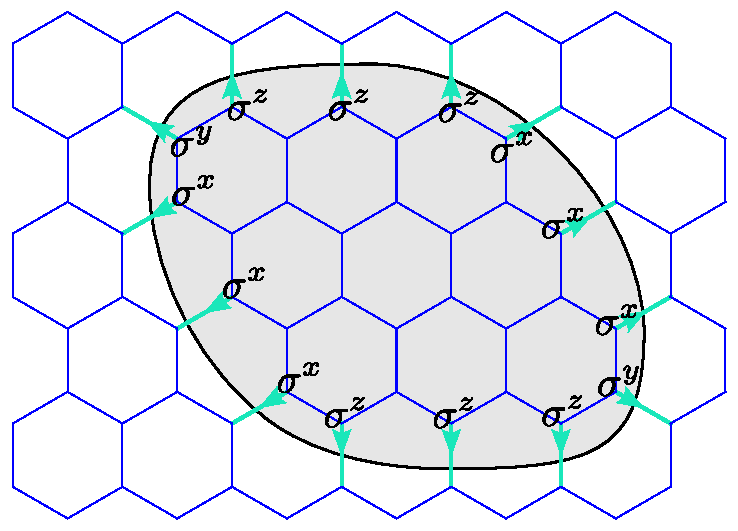
\includegraphics[width=0.24\linewidth]{figures/Yao-Qi-mechanism-origin.pdf}
    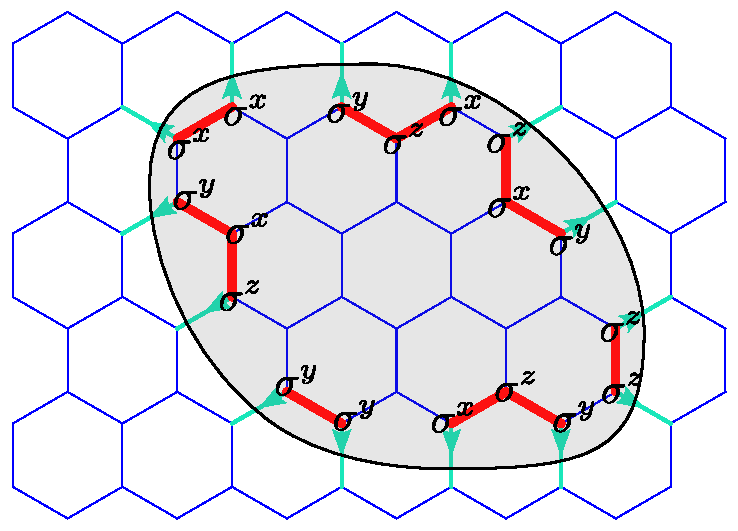
\includegraphics[width=0.24\linewidth]{figures/Yao-Qi-mechanism-dimers.pdf}
    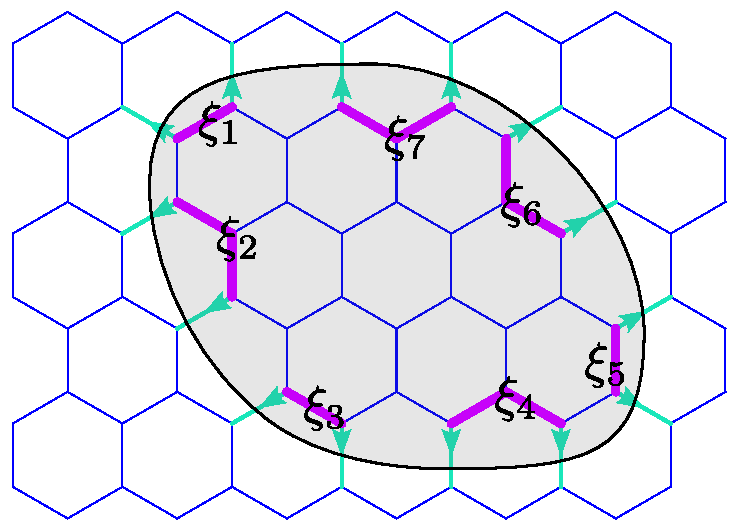
\includegraphics[width=0.24\linewidth]{figures/Yao-Qi-mechanism-xi-def.pdf}
    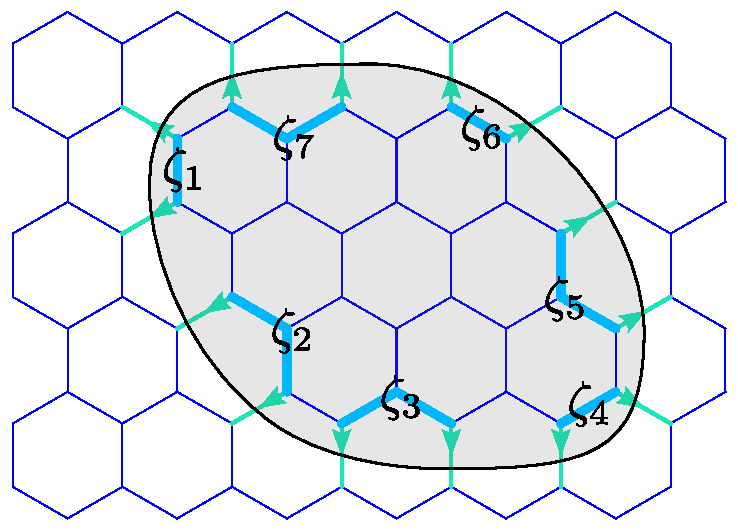
\includegraphics[width=0.24\linewidth]{figures/Yao-Qi-mechanism-zeta-def.pdf}
    \caption{The electric-field operators living on the edges crossing the boundary of the region are split in half, as shown in the first panel. In the physical spin representation, these electric fields correspond to the spin operators $\sigma^\mu$ with directions pointing outwards. The second panel displays string operators that connect two adjacent spins in the first panel in a pair. Multiplying the first panel by the second one gives a series of operators $\xi$, as shown in the third panel. Applying the same method but with the pairing order shifted yields another set of operators $\zeta$, as showcased in the last panel.}
    \label{fig.xi-def}
\end{figure*}
The first three panels of \autoref{fig.xi-def} illustrate an example of the process of defining $\xi$-operators. In the first panel are the spin operators $\sigma^\mu_i$, which are exactly the spin operators shown in equation \eqref{equ.spin-string-linking-gauge}, at the boundary with their directions pointing outwards. In the next panel, we subsequently multiply the string operators $\Sigma_{\mathcal{C}_n}$, which is nothing but the string operator shown in equation \eqref{equ.spin-string-linking-gauge} that lies between the two spin operators residing on the two endpoints of the string, with the spin operators set previously. After that, such operators are used as definitions of $\xi_n$'s, which are illustrated in the third panel of \autoref{fig.xi-def}. In this example, we now focus on $\xi_1$, which is defined as
\[
\xi_1 = \sigma^y_1\lr{\sigma^x_1\sigma^x_2}\sigma^z_2 \propto \sigma_1^z\sigma_2^y.
\]
The subscript ``1'' indicates the lower-left endpoint of the dimer, while ``2'' stands for the other one. It can be shown that $\xi_1$ commutes with every string operator $\Sigma_{\mathfrak{D}}$ with $\mathfrak{D}\subset A$ in a trivial way by examining all possible strings that reach the two endpoints of the dimer where $\xi$ lives. By doing so, one will find that either (i) at one endpoint of a string $\mathcal{C}$, which is right at one of the two endpoints of the $\xi_1$ dimer, is a spin operator whose direction is parallel to the spin operator of $\xi_1$ on that endpoint; Or (ii) none of the two spin operators of $\Sigma_{\mathcal{C}}$, whose positions are the two endpoints of $\xi_1$, is parallel to the spin operator of $\xi_1$ at its position, such that the twice of sign flipping caused by the anti-commutation of Pauli algebra between $\Sigma_{\mathcal{C}}$ and $\xi_1$ gets the positive sign again. These situations, along with the fact that $[\xi_1,W_p]=0\;\forall p$~\footnote{Don't forget that a loop also counts a string, just with two endpoints at the same position. Therefore, proving that every string operator commutes with $\xi_n$ also proves that every plaquette operator commutes with $\xi_n$ at the same time.}, exhaust all the possibilities, allowing us to conclude that $[\xi_1,\rho_A]=0$ because $\rho_A$ consists of plaquette operators and string operators inside $A$, as shown in equation \eqref{equ.red-den-mat-sim-con}. In the same sense, we may generalize this statement to $[\xi_n,\rho_A]=0\;\forall n$, where the operators $\xi_n$ are defined through the process illustrated in \autoref{fig.xi-def} in $A$. At the same time, the regions where $\xi$-operators are supported have no intersection, hence they commute with each other, $[\xi_m,\xi_n]=0\;\forall m,n$. Therefore, the set $\lrg{\xi_1,\cdots,\xi_L}$, with values $\pm 1$, of expectation values of $\xi$-operators defined in $A$ forms good quantum numbers that block-diagonalizes the reduced density matrix $\rho_A$
\begin{equation}\label{equ.rho-block-diagonal-structure}
    \rho_A = \bigoplus_{\lrg{\xi_1,\cdots,\xi_L}} \varrho_{\lrg{\xi_1,\cdots,\xi_L}}
\end{equation}
where each $\varrho_{\lrg{\xi_1,\cdots,\xi_L}}$ is the block labeled by a set of binaries $\lrg{\xi_1,\cdots,\xi_L}$, and thus the number of blocks is $2^{L} = 2^{\abs{\de A}/2}$.

In defining $\xi$-operators, the way we chose to pair points along the boundary was like $(b^{\mu_1}_{i_1},b^{\mu_2}_{i_2}), (b^{\mu_3}_{i_3},b^{\mu_4}_{i_4}),\cdots,(b^{\mu_{2L-1}}_{i_{2L-1}},b^{\mu_{2L}}_{i_{2L}})$. However, it is not the only way to pair these points. We can choose another way in which the pairing order is shifted by one compared to the previous way we adapted for $\xi$-operators
\[
(b^{\mu_2}_{i_2},b^{\mu_3}_{i_3}), (b^{\mu_4}_{i_4},b^{\mu_5}_{i_5}),\cdots,(b^{\mu_{2L}}_{i_{2L}},b^{\mu_1}_{i_1})
\]
and then connect each of them through a new set of strings $\{\mathcal{C}'_n\}$. In this way, a set of operators $\zeta_n$ can be defined
\begin{equation}\label{equ.spin-string-linking-gauge-zeta}
    \zeta_n \equiv \sigma^{\mu_{2n}}_{i_{2n}}\Sigma_{\mathcal{C}'_n}\sigma^{\mu_{2n+1}}_{i_{2n+1}} \quad ; \quad n=1,2,3,\cdots, L
\end{equation}
where the periodic notational convention $i_{2L+1}=i_1$ and $\mu_{2L+1}=\mu_1$ is used. In the same sense, these $\zeta$-operators also commute with the reduced density matrix. An example of a set of $\zeta$-operators is illustrated in the fourth panel of \autoref{fig.xi-def}, from which we can see that the pattern of $\zeta$-operators differs from that of $\xi$-operators by shifting a unit along the boundary, so that each $\xi_n$ is in between $\zeta_{n-1}$ and $\zeta_n$. According to the algebraic rules of Pauli matrices, a relation between $\xi$-operators and $\zeta$-operators can be obtained directly
\begin{equation}\label{equ.xi-zeta-relation}
    \zeta_n\xi_m\zeta_{n} =
\left\{
\begin{array}{ll}
   -\xi_m &;\; \text{for $m=n\vee n+1$} \\
   \xi_m  &;\; \text{otherwise} 
\end{array}
\right.
\end{equation}
This equation implies that the $\zeta$-operators relate different blocks of the density matrix $\rho_A$ in the way that
\begin{equation}\label{equ.related-blocks}
    \zeta_n \varrho_{\lrg{\cdots,\xi_n,\xi_{n+1},\cdots}}\zeta_n = \varrho_{\lrg{\cdots,-\xi_n,-\xi_{n+1},\cdots}}
\end{equation}
By this relation, any two blocks $\varrho_{\lrg{\xi}}$ and $\varrho_{\lrg{\xi'}}$ in $\rho_A$ can be related, and thus their sets of eigenvalues are identical. However, a $\zeta$-operator flips the eigenvalues of two $\xi$-operators at the same time, so it is not quite correct to say any two blocks can be related through applying $\zeta$-operators. Considering this simultaneous flipping of two quantum numbers, the statement should be modified to: Two blocks, $\varrho_{\lrg{\xi}}$ and $\varrho_{\lrg{\xi'}}$, are related by a specific set of $\zeta$-operators only when they have the same total parity, $\prod_{i=1}^{L}\xi_i = \prod_{i=1}^{L}\xi'_i$, defined by multiplying every quantum number in $\lrg{\xi}$.

So far, we have had a better understanding of the block-diagonal structure of $\rho_A$, and now we are going to discuss the origin of the degeneracy in the entanglement spectrum, as well as another point of view of the contribution of the gauge field to the entanglement entropy. Based on the block-diagonal structure \eqref{equ.rho-block-diagonal-structure} of $\rho_A$ and the fact that $\zeta$-operators can relate different blocks to prove them identical, we then conclude that there are 
\[2^{L-1} = 2^{\abs{\de A}/2 - 1}\] 
identical blocks in $\rho_A$. The reason why we only have the number $2^{L-1}$ instead of $2^L$, which is the number of blocks in \eqref{equ.rho-block-diagonal-structure}, is that $\zeta$-operators can only relate blocks with the same parity of the set of quantum numbers $\lrg{\xi}$, so the number of blocks, $2^L$, is actually twice the number of identical blocks. The factor $2^{-1}$ arising from the fixed parity of quantum numbers can also be understood as originating from the exact 1-form Wilson symmetry~\cite{PRX-ent-high}, which is $[\Tilde{W}_h,H] = [\Tilde{W}_v,H] = [W_p,H]=0\;\forall p$. After tracing out the environment $\overline{A}$, the global Wilson operator in the sense of merely the subregion $A$ becomes a string with two endpoints attached to the boundary of $A$, and commutes with $\rho_A$ at the same time. The two endpoints of the Wilson operator can flip the residual $\mathbb{Z}_2$ gauge field at the boundary, playing a role in relating different blocks of $\rho_A$. This is completely the same as the $\zeta$-operators. Based on the block-diagonal structure of $\rho_A$, it can be expressed as
\begin{equation}\label{equ.block-rho-final}
    \rho_A = \bigoplus_{n=1}^{2^{L-1}}\varrho^{(n)}_A
\end{equation}
with all the blocks $\varrho_A^{(n)}$ identical. Substitution of such an expression into the definition of von Neumann entropy directly gives the entanglement entropy, 
\begin{align}\label{equ.EE-from-blocks}
    S_A 
    &= -\Tr_A\rho_A\ln\rho_A \nonumber \\
    &= -\Tr_A\lrm{\bigoplus_{n=1}^{2^{L-1}}\lr{\varrho^{(n)}_A \ln \varrho^{(n)}_A}} \nonumber \\
    &= -2^{L-1}\Tr_A\varrho_A \ln \varrho_A \nonumber \\
    &= -\Tr_A\Tilde{\rho}_A\ln\Tilde{\rho}_A + \lr{\frac{1}{2}\abs{\de A} -  1}\ln 2
\end{align}
where $\Tilde{\rho}_A \equiv 2^{L-1}\varrho_A$ is the normalized density matrix
defined to make $\Tr_A\Tilde{\rho}_A=1$. By comparing Eq.~\eqref{equ.EE-from-blocks} with Eq.~\eqref{equ.EE-separation}, we find that each block $\Tilde{\rho}_A$ corresponds to the Majorana reduced density matrix $\rho_A^F$. At the same time, the gauge part $S^G_A$ can be understood as a measure of the number of identical blocks in $\rho_A$, which is exactly the degree of degeneracy in the entanglement spectrum. This agrees with the gauge nature of such a contribution since the degeneracy arises from the block-diagonal structure of $\rho_A$ along with the fact that every block is identical, and the presence of block-diagonal structure is due to the residual electric field from the Gauss law after the environment is traced out. Notice that the residual Gauss law does not purely cause the degeneracy in the entanglement spectrum. Instead, it also has things to do with the existence of $\zeta$-operators, through which all blocks can be related. Finally, the topological entanglement entropy $-\ln 2$ is a consequence of the constraint that the total parity of the quantum numbers, $\prod_{n=1}^L\xi_n$, is fixed, and its origin lies in the existence of the 1-form Wilson symmetry, which satisfies our earlier understanding about the topological entanglement entropy. The most important thing is that the full entanglement spectrum of the Kitaev ground state is obtained. Since an entanglement spectrum is defined as the spectrum of a reduced density matrix, formula \eqref{equ.block-rho-final} directly answers that the entanglement spectrum is the eigenvalue spectrum of $\varrho_A$ with $2^{\abs{\de A}/2-1}$-fold degeneracy. As shown by the comparison between \eqref{equ.EE-from-blocks} and \eqref{equ.EE-separation}, we know that the block $\varrho_A$ is proportional to the Majorana fermion density matrix $\rho^F_A$, and whose spectrum can be solved exactly using the method proposed in Ref.~\cite{Jin-Korepin, Vidal-Latorre-Rico-Kitaev, Latorre-Rico-Vidal, Peschel_2003, Peschel_2009, Chung_2001, Cheong_2004}.

From a more fundamental point of view, the set of $\xi$-operators block-diagonalizes every string operator in a way identical to what we have for $\rho_A$ because each of them commutes with every string operator, and hence so is $\mathcal{S}^{(A)}_{\mathfrak{D}}$
\[
[\xi_i,\mathcal{S}^{(A)}_{\mathfrak{D}}]=0 \;\forall i\in\lrg{1,2,\cdots,L}
\]
Similar to equation \eqref{equ.block-rho-final}, every $\mathcal{S}$-operator can also be block-diagonalized as
\begin{equation}\label{equ.U-V-block-relation}
    \mathcal{S}^{(A)}_{\mathfrak{D}} = \bigoplus_{n=1}^{2^{L-1}}\mathcal{M}^{(n)}_{\mathfrak{D}}
\end{equation}
where $\{\mathcal{M}^{(n)}_\mathfrak{D}\}$ is a set of identical blocks of $\mathcal{S}^{(A)}_{\mathfrak{D}}$. To ensure that expression \eqref{equ.U-V-block-relation} satisfies rule \eqref{equ.U-rep-algebra}, we also have to implement such an algebraic rule on every block $\mathcal{M}^{(n)}_{\mathfrak{D}}$, 
\[
\mathcal{M}^{(n)}_{\mathfrak{D}}\mathcal{M}^{(n)}_{\mathfrak{D}'} = g(\mathfrak{D},\mathfrak{D}')\mathcal{M}^{(n)}_{\mathfrak{D}\oplus\mathfrak{D}'}
\]
This is reminiscent of \eqref{equ.V-rep-algebra}, which shows that the $\mathcal{M}$-representation is identical to $\mathcal{S}$. Based on this, we then state that those blocks $\mathcal{M}^{(n)}_{\mathfrak{D}}$ in \eqref{equ.U-V-block-relation} are nothing but $\mathcal{M}$-operators defined in \eqref{equ.V-rep-def}. In short, the gauge-field degree of freedom is actually the number of identical blocks of string operators represented by spins, and each identical block depicts the physics of free Majorana fermions. This precisely reflects the fractionalization of the spin degree of freedom into gauge-field and matter sectors, with the matter sector further fractionalizing into deconfined Majorana fermions.


\begin{figure*}
    \centering
    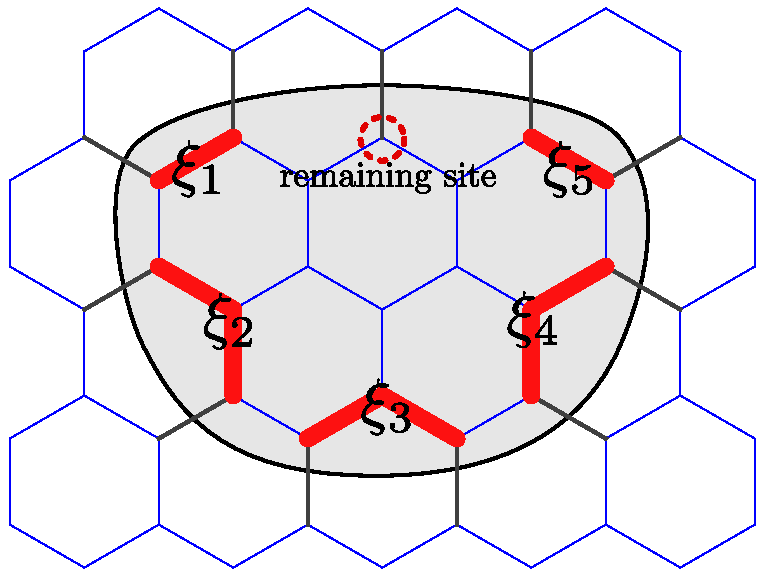
\includegraphics[width=0.25\linewidth]{figures/reshuffle-xi-def-odd.pdf}\hspace{0.5cm}
    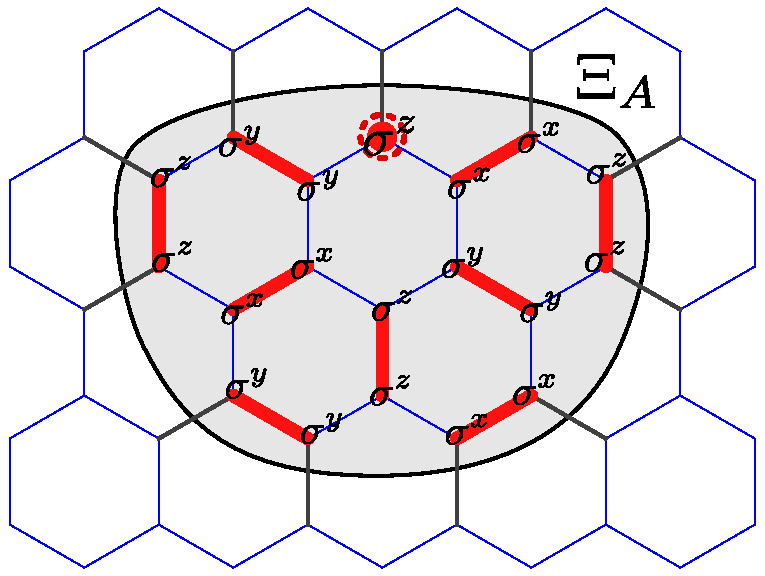
\includegraphics[width=0.25\linewidth]{figures/reshuffle-capital-Xi-def.pdf}\hspace{0.5cm}
    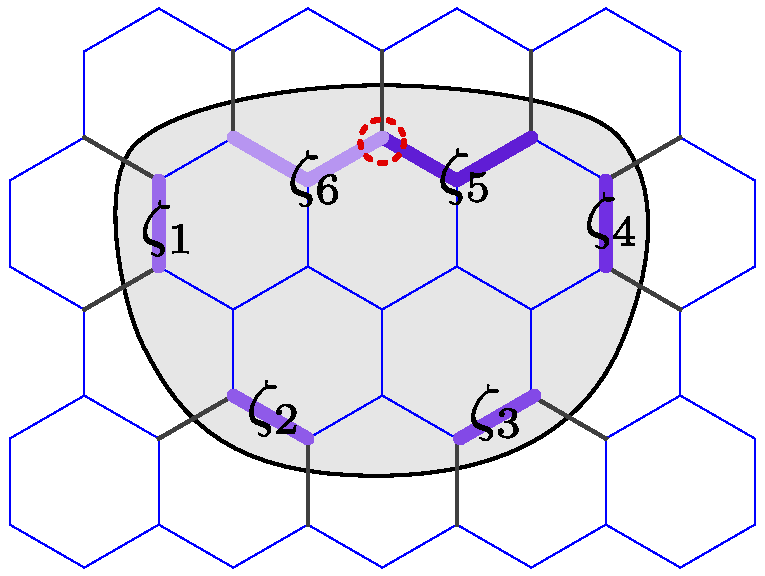
\includegraphics[width=0.25\linewidth]{figures/reshuffle-zeta-def-odd.pdf}
    \caption{For cases with odd $N^A$, there must be a single site $l$ on the boundary that remains unpaired after defining $\xi$-operators by pairing the adjacent edges crossing the boundary, as illustrated in the left-most panel. Based on this phenomenon, we can define an operator $\Xi_A$ in such a way that the remaining site $l$ is filled in with a Pauli matrix $\sigma^\mu_l$, where $\mu$ is the direction of the edge crossing the boundary that connects to $l$. At the same time, the rest of the part is covered by a dimer covering, as illustrated in the middle panel. On the other hand, the $\zeta$-operators are defined in a way similar to what we have introduced, but there are two connected $\zeta$-operators sharing one site, which is exactly $l$ after the pairing we have done to define $\xi$-operators. In the example illustrated in the right-most panel, the two connected $\zeta$-operators are $\zeta_5$ and $\zeta_6$, and we have $\zeta_5\Xi\zeta_5 = \zeta_6\Xi_A\zeta_6 = -\Xi_A$.}
    \label{fig.Xi-odd}
\end{figure*}
In the above discussion, everything is well-defined since $\abs{\de A}$ was set to be even. In that case, the sites along the boundary can be sorted into pairs to define a set of $\xi$-operators that link two sites in a pair. However, as shown by relation \eqref{equ.bulk-boundary-parity}, once the number of lattice sites in $A$ is odd, so is the length of the boundary. This raises an issue that there will always be one single site that remains after sorting lattice sites along the boundary in pairs, as shown in the first panel of \autoref{fig.Xi-odd}. If $L$ is defined as the number of $\xi$-operators, then in cases with odd $\abs{\de A}$, we have
\[
L = \frac{1}{2}\lr{\abs{\de A} - 1}
\]
In this way, the block-diagonal structure \eqref{equ.block-rho-final} and the derivation \eqref{equ.EE-from-blocks} are still valid, but the result should be modified as
\begin{align}\label{equ.EE-odd-blocks}
    S_A &= -\Tr_A\Tilde{\rho}_A\ln\Tilde{\rho}_A + \lr{L-1}\ln 2 \nonumber\\
    &= -\Tr_A\Tilde{\rho}_A\ln\Tilde{\rho}_A + \lr{\frac{1}{2}\abs{\de A}-\frac{3}{2}}\ln 2
\end{align}
where $\Tilde{\rho}_A\equiv 2^{L-1}\varrho_A$. The form of \eqref{equ.EE-odd-blocks} is the same as that of \eqref{equ.EE-odd-derive-1}, showing that the block $\Tilde{\rho}_A$ here is identical to the Majorana reduced density matrix \eqref{equ.rho-A-F-odd} with a redundant Majorana fermion included. 

In Section~\ref{sec:EE-calculation-odd}, the result of the Majorana entanglement spectrum shows that the degree of degeneracy is 
\[
2^{\frac{N^A+1}{2}-N^A_p} = 2^{\frac{1}{2}\lr{\abs{\de A} - 1}} = 2^L
\]
However, according to the discussion in the previous part for cases with an even number of sites, the degree of degeneracy is $2^{L-1}$ if there are $L$ well-defined $\xi$-operators. This discrepancy between counting the number of $\xi$-operators and analyzing the degree of degeneracy according to the Majorana entanglement spectrum implies that, apart from the set of $\xi$-operators, there exists an additional operator that further block-diagonalizes $\rho_A$ to give an additional 2-fold degeneracy to the entanglement spectrum. At the end of Section~\ref{sec:EE-calculation-odd}, we have elucidated that the additional 2-fold degeneracy in the entanglement spectrum of the Majorana sector originates from the total fermion parity, in the sense that $\rho_A$ is further block-diagonalized into two identical blocks by $\hat{\bog{\pi}}^{(A)}$, corresponding to even and odd, respectively. Therefore, we anticipate that the additional operator, which will be denoted by $\Xi_A$ later on, is related to the total fermion parity in the Majorana representation. A feasible choice is a dimer covering of the subregion $A$. In that matter, $\Xi_A$ is defined as
\begin{equation}\label{equ.Xi-def}
    \Xi_A \equiv \sigma^\mu_l \prod_{\anglelr{ij}\in\mathfrak{D}_{\mrm{DC}}^{A(l)}}\dimer{i}{j}
\end{equation}
The edge configuration $\mathfrak{D}_{\mrm{DC}}^{A(l)}$ stands for a dimer covering of $A$ with a site $l$ being excluded. Since $N^A$ is an odd number, it is not possible for a dimer configuration composed of non-overlapping dimers to cover the entire subregion. The dimer covering is not uniquely defined. A dimer configuration can be arbitrarily chosen as long as $\Xi_A$ gives the 2-fold degeneracy in the entanglement spectrum. The remaining site $l$ is required to be at the boundary of the subregion $A$, which will be explained later, and at which the direction $\mu$ of the Pauli matrix $\sigma_l^\mu$ is that of the edge connected to $l$ that crosses the boundary. An example is illustrated in \autoref{fig.Xi-odd}, where the remaining site $l$ is in the upper portion of the subregion. 

$\Xi_A$ can be examined to commute with $\rho_A$ in the same way as used for $\xi$-operators. String operators are composed of multiple dimers, and every dimer commutes with the dimer covering because of the properties of Pauli matrices. Therefore, the only thing to be concerned about is $\sigma^\mu_l$ lying at the remaining site.
As we have defined, the site $l$ is at the boundary and $\mu$ points outward, it can be seen directly that, inside $A$, there are only two edges connected to $l$, and the corresponding string operator of both edges anti-commutes with $\sigma^\mu_l$. However, since the string operator also anti-commutes with the dimer that connects to the other endpoint of the edge, the two anti-commutations cancel each other. In the end, every string operator with $\mathfrak{D}\subset A$ commutes with $\Xi_A$. Finally, because $\rho_A$ is composed of string operators inside $A$, we conclude that $[\Xi_A,\rho_A]=0$. 

It would be transparent to see that $\Xi_A$ is related to the total fermion parity by transforming \eqref{equ.Xi-def} into the Majorana fermion representation, and we find that it is equal to the total fermion parity operator multiplied by the gauge-field operators arranged in order of the dimer covering $\mathfrak{D}^{A(l)}_{\mrm{DC}}$
\[
\Xi_A \propto \lr{\prod_{\anglelr{ij}\in  \mathfrak{D}^{A(l)}_{\mrm{DC}}} \hat{u}_{ij}} \lr{b^\mu_l\prod_{i\in A}c_i}
\]
up to a phase. In the above formula, the total fermion parity operator is defined as
\begin{equation}\label{equ.total-fermion-parity-odd}
    \hat{\bog{\pi}}^{(A)} \propto b^\mu_l\prod_{i\in A}c_i
\end{equation}
with a phase correction depending on the geometry of the subregion. Because the gauge has been fixed as $u_{ij}=1\;\forall\anglelr{ij}$, the expectation value of $\Xi_A$ is completely determined by that of $\hat{\bog{\pi}}^{(A)}$. The definition of the total fermion parity here is different from what we encountered in \eqref{equ.total-fermion-parity-entire-system} and \eqref{equ.total-fermion-parity-Sigma-Z}. In fact, it is due to $N^A$ being an odd number, so that $\prod_{i\in A}c_i$ itself only contains an odd number of Majorana fermions, hence not sufficient to define a fermion parity operator. This mechanism has been discussed in Section~\ref{sec:EE-calculation-odd}, and the alternative we adopted there is to include a redundant Majorana fermion $c_{(N^A+1)}$. In \eqref{equ.total-fermion-parity-odd}, it can be seen that the redundant fermion is in fact $b^\mu_l$ borrowed from the gauge sector. The situation in which the $c$-Majorana sector borrows a Majorana fermion from the gauge sector is also demonstrated in the derivation procedures \eqref{equ.EE-odd-derive-1} and \eqref{equ.EE-reduce}. By now, the physical meaning of the redundant fermion and its origin are clearly reflected by $\Xi_A$. 

So far, we have $L$ distinct $\xi$-operators and $\Xi_A$ that commute with $\rho_A$. These operators give $2^{L+1}$ blocks labeled with a set of eigenvalues $\lrg{\xi_1,\cdots,\xi_L;\Xi_A}$. To prove that these blocks are identical, leading to extensive degeneracy, we also have to find $(L+1)$ $\zeta$-operators that relate all the blocks in the same way as \eqref{equ.xi-zeta-relation}. In the line of defining $\xi$-operators, we can only define $L$ $\zeta$-operators. However, it turns out that we can still find $(L+1)$ $\zeta$-operators since they are not required to commute with each other. As illustrated in the last panel of \autoref{fig.Xi-odd} the arrangement of $\zeta$-operators is designed in such a way that two of them overlap at the remaining site $l$. In this way, the $\xi$-operators can still be flipped through \eqref{equ.xi-zeta-relation}. More importantly, both overlapping $\zeta$-operators can flip the sign of $\Xi_A$. In \autoref{fig.Xi-odd}, these two operators are $\zeta_5$ and $\zeta_6$, by which $\Xi_A$ can be flipped in the way that $\zeta_5\Xi_A\zeta_5 = \zeta_6\Xi_A\zeta_6 = -\Xi_A$. In all, the situation here is similar to what we encountered in cases with even $N^A$, in which each $\zeta$-operator simultaneously flips two values in the set $\lrg{\xi_1,\cdots,\xi_L;\Xi_A}$. Therefore, although we have $2^{L+1}$ operators to block-diagonalize $\rho_A$, they only provide $2^L$-fold degeneracy in the entanglement spectrum. This agrees with our analysis in Section~\ref{sec:EE-calculation-odd}, and the operator $\Xi_A$ indeed gives a 2-fold degeneracy to the entanglement spectrum. 

It seems that $\Xi_A$ can also be defined in cases with even $N^A$ as illustrated in \autoref{fig.dimer-covering}, and gives a 2-fold degeneracy as well.
\begin{figure}
    \centering
    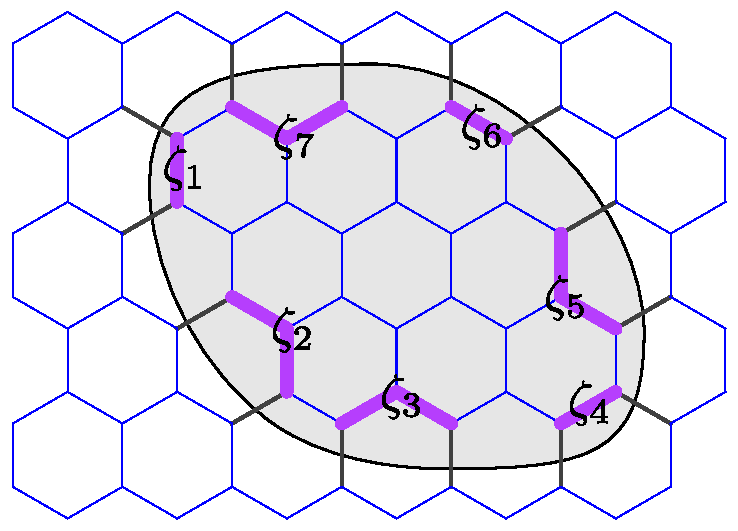
\includegraphics[width=0.4\linewidth]{figures/reshuffle-larger-zeta.pdf}\hspace{0.5cm}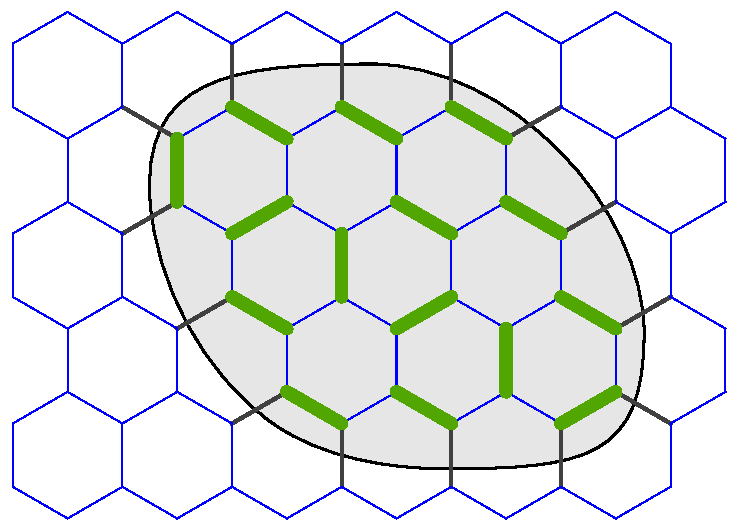
\includegraphics[width=0.4\linewidth]{figures/reshuffle-larger-dimer-covering.pdf}
    \caption{For regions with an even number of lattice sites, at least a dimer covering is well defined, like the one illustrated in the right panel. Assigning a string operator to each dimer in the configuration gives a dimer-covering string operator $\Xi_A$ without a single unpaired site, unlike we encountered in cases with an odd number of sites. However, it can be directly checked that $\Xi_A$ in this case commutes with every $\zeta$-operator. Therefore, such an operator doesn't provide additional degeneracy in the entanglement spectrum.}
    \label{fig.dimer-covering}
\end{figure}
In this case, the pattern is simply a dimer covering without a remaining site. However, $\Xi_A$ defined in this case commutes with every $\zeta$-operator, implying that no operator can relate blocks with $\Xi_A=+1$ to $\Xi_A=-1$ and vice versa. Thus, $\Xi_A$ cannot provide a 2-fold degeneracy in the entanglement spectrum in cases with even $N^A$. This constitutes an intrinsic difference between cases with even and odd $N^A$, which is reflected in the total fermion parity in the subregion in the Majorana representation, or equivalently in the dimer covering operator $\Xi_A$ in the physical spin formulation.

